The cell noise for the reprocessed data has been calculated in the different
gain combinations. In
\cref{fig:noise_avg_hghg,fig:noise_avg_lglg,fig:noise_avg_hglg} the cell noise
values have been calculated using all the calibration runs used for the 2011 RUN
I reprocessing, each fitted using the optimal filtering method (see
\cref{sec:optimal-filtering}). The plots show the $\eta$--dependence of the
$\phi$--averaged RMS of the noise in these runs. Each point is an average for a
given cell over all modules containing this cell type. This is done for a given
gain combination of the readout channels: High Gain--High Gain
(\cref{fig:noise_avg_hghg}), Low Gain--Low Gain (\cref{fig:noise_avg_lglg}) or
High Gain--Low Gain (\cref{fig:noise_avg_hglg}). The plots separate the
different cell types: A, BC, D and E (gap and crack scintillators). Note that
gap and crack scintillators have only one readout channel, so are plotted only
in HG or LG readout. The transition between the long and extended barrels can be
seen in the range $0.7 < |\eta| < 1.0$.
\begin{figure}[!h]
  \centering
    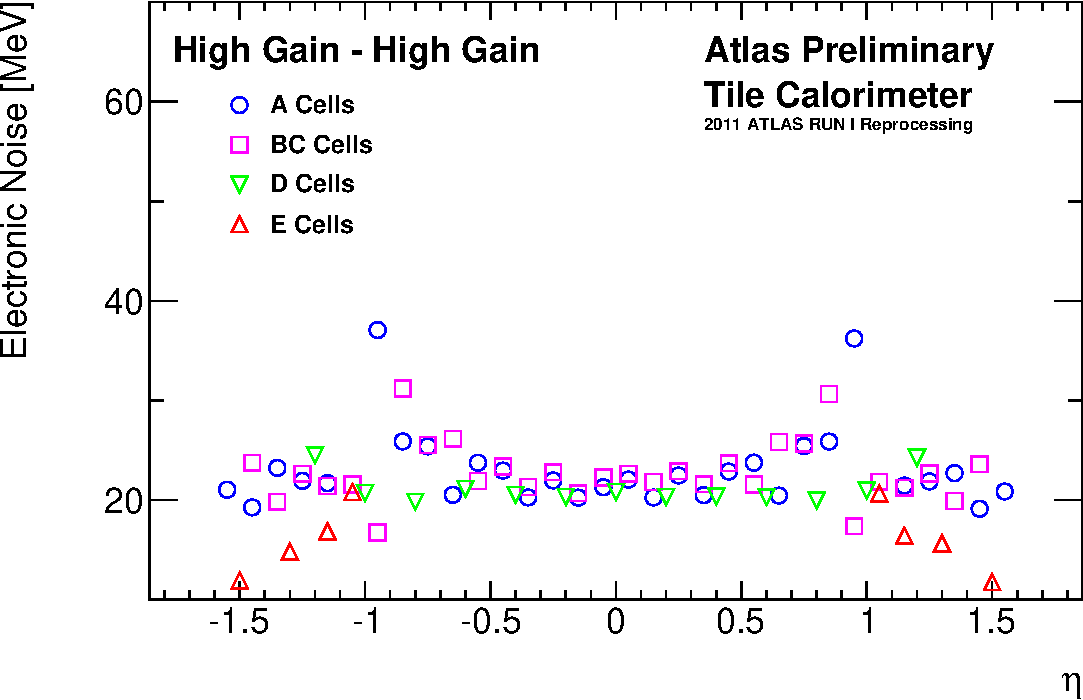
\includegraphics[width=.8\linewidth]{noise_avg_hghg}
    \caption{$\phi$--averaged RMS of electronic cell noise as a function of
      $\eta$ of the cell, with both readout channels in High Gain. For each cell
      the average value over all modules is taken. Values have been extracted
      using all the calibration runs used for the 2011 RUN I reprocessing. The
      different cell types are shown separately, A, BC, D, and E
      (gap/crack). The transition between the long and extended barrels can be
      seen in the range $0.7 < |\eta| < 1.0$. HGHG combination is relevant when
      the energy deposition in the cell is
      $\lesssim 15$~GeV~\cite{MyTileCalPlots}.}
    \label{fig:noise_avg_hghg}
\end{figure}

\begin{figure}[!h]
  \centering
    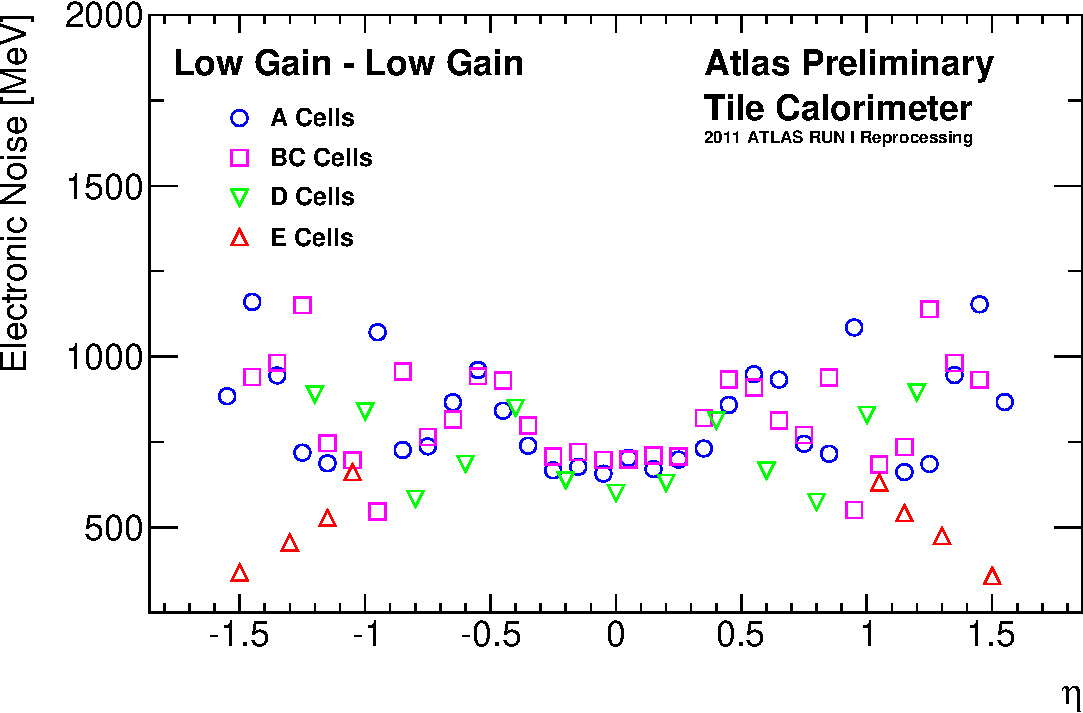
\includegraphics[width=.8\linewidth]{noise_avg_lglg}
    \caption{$\phi$-averaged RMS of electronic cell noise as a function of
      $\eta$ of the cell, with both readout channels in Low Gain. For each cell
      the average value over all modules is taken. Values have been extracted
      using all the calibration runs used for the 2011 RUN I reprocessing. The
      different cell types are shown separately, A, BC, D, and E
      (gap/crack). The transition between the long and extended barrels can be
      seen in the range $0.7 < |\eta| < 1.0$. LGLG combination is relevant when
      the energy deposition in the cell is
      $\gtrsim 15$~GeV~\cite{MyTileCalPlots}.}
    \label{fig:noise_avg_lglg}
\end{figure}

\begin{figure}[!h]
  \centering
    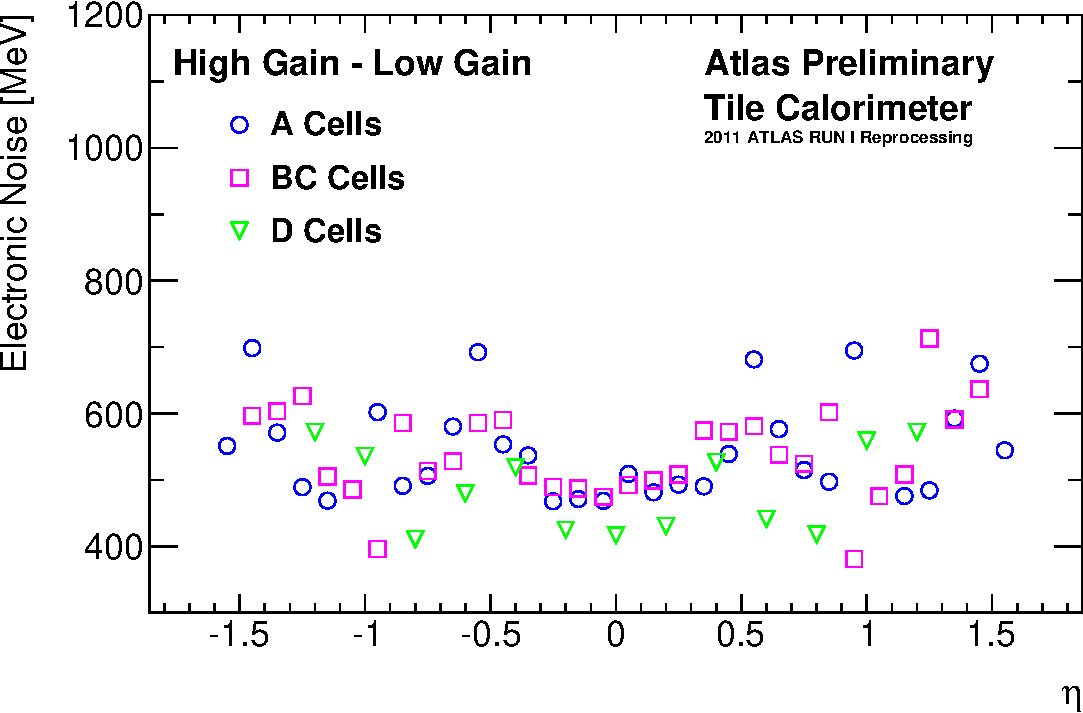
\includegraphics[width=.8\linewidth]{noise_avg_hglg}
    \caption{$\phi$-averaged RMS of electronic cell noise as a function of
      $\eta$ of the cell, with one readout channel in High Gain and the other in
      Low Gain. For each cell the average value over all modules is
      taken. Values have been extracted using all the calibration runs used for
      the 2011 RUN I reprocessing. The different cell types are shown
      separately, A, BC, D. E cells do not appear int this plot since they have
      only one readout channel. The transition between the long and extended
      barrels can be seen in the range $0.7 < |\eta| < 1.0$. When the energy
      deposition in the cell is between 10~GeV $\lesssim E \lesssim$ 20~GeV it
      can happen that the cell is read out with different voltage on the readout
      channels~\cite{MyTileCalPlots}.}
    \label{fig:noise_avg_hglg}
\end{figure}

\cref{fig:noise_avg_hghg,fig:noise_avg_lglg,fig:noise_avg_hglg} exhibit some
$\eta$--dependence of the noise. There are two main factors behind this, first
the low voltage power supplies, which are the main noise source in TileCal, are
located approximately at $|\eta| \approx 1$ leading to higher noise in the cells
in that region. Secondly the noise in these plots is in MeV, cells with the same
noise expressed in ADC counts can have different noise levels when converted in
MeV. This is due to the different ADC to GeV calibration factors for cells with
different geometries.
% Figures 5.5 to 5.exhibit some eta-dependence of the noise. There are two main
% factors behind this, first the low voltage power supplies are known to be the
% main source of noise in TileCal, they are located at |eta|~1 and lead to higher
% noise in the cells in that region.  Secondly the noise in these figures is shown
% in MeV. Two channels with the same noise expressed in ADC counts can have
% different noise levels expressed in MeV as two cells with different geometries
% will have different ADC to GeV calibration factors.
%%% Local Variables:
%%% mode: latex
%%% TeX-master: "../search_for_DM_LED_with_ATLAS"
%%% End:
